%%%%%%%%%%%%%%%%%%%%%%%%%%%%%%%%%%%%%%%%%%%%%%%%%%%%%%%%%%%
%%%%% 													%%%%%
%%%%%	Aller voir le lien suivant :					%%%%%
%%%%%													%%%%%
%%%%%	http://fr.wikibooks.org/wiki/LaTeX				%%%%%
%%%%%													%%%%%
%%%%%%%%%%%%%%%%%%%%%%%%%%%%%%%%%%%%%%%%%%%%%%%%%%%%%%%%%%%

\documentclass[a4paper,12pt]{report}

%%%%%%%%%%%%%%%%%%%%%%%%%%%%%%%%%%%%%%%%%%%%%%%%%%%%%%%%%%%
%%%%% 	pour le français et les accents 	      %%%%%
%%%%%%%%%%%%%%%%%%%%%%%%%%%%%%%%%%%%%%%%%%%%%%%%%%%%%%%%%%%

\usepackage[utf8]{inputenc} 
\usepackage[french]{babel} 

%%%%% 		Pour les marges de la page			 %%%%%%%%
\usepackage[top=2cm, bottom=2cm, left=2cm, right=2cm]{geometry}
%%%%%%%%%%%%%%%%%%%%%%%%%%%%%%%%%%%%%%%%%%%%%%%%%%%%%%%%%%%


\usepackage[T1]{fontenc}

%%%%% Pour les url %%%%%
\usepackage{hyperref}

%%%%% Gestion des numeros de sous-sous-sections %%%%%
\usepackage{titlesec}
\setcounter{secnumdepth}{3}

%%%%% Gestion des sous sous section dans la TOC %%%%%
\setcounter{tocdepth}{3}

%%%%% Insertion des images %%%%%
\usepackage{graphicx}

%%%%% Gestion du centrage des titres %%%%%
\usepackage{sectsty}
\usepackage{lipsum}

%%%%% Demarrage à 0 des sections %%%%%%
\renewcommand{\thesection}{\arabic{section}}
\setcounter{section}{0}


%%% Maketitle metadata
\newcommand{\horrule}[1]{\rule{\linewidth}{#1}} 	%ligne horizontale

\parindent=1cm

%%% Forcer les images à rester dans leur section
\usepackage[section]{placeins}


%%%%%%%%%%%%%%%%%%%  PAGE DE GARDE %%%%%%%%%%%%%%%%%%%%%%
\title{	
		\horrule{0.5pt} \\[0.5cm]
		\huge PJI Architecture TOR sur\\ navigateur web \\
		\horrule{0.5pt} \\[0.5cm]
}
\author{
		\normalfont 								\normalsize
        Franquenouille Kevin\\[-3pt]		\normalsize
       	Cornette Damien\\[-3pt]		\normalsize
       	Git Repository : \url{https://github.com/kfranquenouille/PJI-TOR.git} \\[-3pt]		\normalsize
}
\date{
		\normalfont 								\normalsize
        Année universitaire : 2014-2015\\[-3pt]		\normalsize
}

%%%%%%%%%%%%%%%%%%%  DEBUT DU RAPPORT %%%%%%%%%%%%%%%%%%%%
\begin{document}

\maketitle	

%%%%%%%%%%%%%%%%%%%  DEBUT INTRODUCTION %%%%%%%%%%%%%%%%%%%%
\newpage
\begin{center}
\section*{Introduction}
\end{center}
\paragraph{}
Tor est un projet pour le support de l'anonymat en dissimulant les communications entre un client web et un serveur. Le mécanisme s'appuie sur un ensemble de relais de confiance disposés sur des serveurs. 
\paragraph{} 
Le nombre limité de relais (moins de 5000) et la confiance dans leur non-compromission peut être considéré comme une limitation de l'approche de Tor. Un moyen d'outrepasser cette limitation serait de limiter le rôle du serveur a un simple relais et de laisser les clients gérer l'anonymat dans le système. 
\paragraph{}
Afin de rendre le système le plus pratique et adoptable pour multiplier les chemins possibles, une idée serait de ne s'appuyer que sur des technologies webs (http, javascript) pour que chaque navigateur puisse devenir un client.
\paragraph{}
Le but de ce projet est d'étudier la faisabilité de l'approche à l'aide de technologie comme websocket. Le cas d'étude sera limité à un simple chat (saisie limitée à 140 caractères).

%%%%%%%%%%%%%%%%%%%  FIN INTRODUCTION %%%%%%%%%%%%%%%%%%%%

%%%%%%%%%%%%%%%%%%%  DEBUT TABLE DES MATIERES %%%%%%%%%%%%%%%%%%%%
\tableofcontents
%%%%%%%%%%%%%%%%%%%  FIN TABLE DES MATIERES %%%%%%%%%%%%%%%%%%%%

%%%%%%%%%%%%%%%%%%%  DEBUT %%%%%%%%%%%%%%%%%%%%
\newpage
\section{Description générale du projet}
	\subsection{Problématique}
	\paragraph*{}
	Le but de ce projet était de mettre en place une "simulation" du réseau TOR via un navigateur web. Pour cela, nous avons pu voir avec Julien Iguchi-Cartigni les technologies que l'on pouvait utiliser. De ce fait, on a pu découpé le projet en 2 parties : 
	\begin{itemize}
		\item[•] Web Cryptography API
		\item[•] WebSocket API
	\end{itemize}
	\paragraph*{}
	Pour réaliser cela, nous devions réaliser cela avec un seul relais client pour debuter puis ensuite le faire avec 3 afin de bien vérifier l'encryption des messages et que les messages sont bien redirigés vers le prochain relais.
	\begin{figure}[h] %%%%% h = here, t = top, b = bottom
		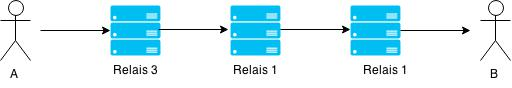
\includegraphics[scale=0.8]{project.jpg}
		\caption{Transfert d'un message de A vers B en passant par 3 relais}
		\label{project}
	\end{figure}
	
	\subsection{Web Cryptography API}
	\paragraph*{}
	Afin de bien crypter les messages envoyés et d'utiliser une technologies assez fiable et récente, nous avons privilégié cette API. En effet, elle est compatible sur presque tous les navigateurs (inclus de base). En revanche, il nous a fallu trouver un bon algorithme de chiffrement.\\
	Dans un premier temps, nous avons utilisé le chiffrement AES-CBC afin de tester et découvrir Webcrypto API et réaliser un premier jet de ce que nous voulions faire. Une fois le messages encrypté 4 fois. Voici un exemple du cryptage :
	\newpage	
	\begin{figure}[h] %%%%% h = here, t = top, b = bottom
		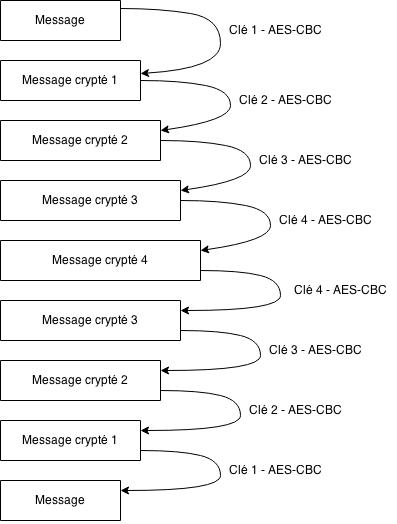
\includegraphics[scale=0.70]{AES.jpg}
		\caption{Cryptage d'un message 4 fois de suite en AES-CBC}
		\label{AES}
	\end{figure}
	\paragraph*{}
	Pour la solution optimale, il est plus préférable d'utiliser un système de clés publiques et de clés privées. Avec l'algorithme RSA-OAEP, celà est possible. Chaque clé générée (l'objet KeyPromise) contient une clé publique et une clé privée. De ce fait, cette solution est plus attendu car elle ressemble très fortement à l'architecture du réseau TOR. Bien entendu, le client doit connaître le chemin afin qu'il puisse créer son message crypté avec les clés publiques des relais correspondants.
	
	\subsection{WebSocket API}

	\subsection{Architecture de l'application}

\newpage	
\section{Mode d'emploi}
	\subsection{Installer un relais}
	
	\subsection{Configurer un relais}
	
	\subsection{Configurer un client}

	\subsection{Lancer l'application}
	
\newpage	
\section{Tests}
	\subsection{Docker}
	
	\subsection{Cryptographie}
	
	\subsection{WebSocket}

\newpage	
\begin{center}
\section*{Conclusion}
\end{center}
\end{document}